\documentclass[twocolumn,english]{article}
\usepackage[latin9]{inputenc}
\usepackage[landscape]{geometry}
\geometry{verbose,tmargin=0.5in,bmargin=0.75in,lmargin=0.5in,rmargin=0.5in}
\setlength{\parskip}{0bp}
\setlength{\parindent}{0pt}
\usepackage{float}
\usepackage{booktabs}
\usepackage{graphicx}

\makeatletter

\providecommand{\tabularnewline}{\\}

\setlength{\columnsep}{0.25in}
\usepackage{xcolor}
\usepackage{textcomp}
\usepackage{listings}
\lstset{
  language=haskell,
  tabsize=2,
  basicstyle=\small\ttfamily,
}

\@ifundefined{showcaptionsetup}{}{%
 \PassOptionsToPackage{caption=false}{subfig}}
\usepackage{subfig}
\makeatother

\usepackage{babel}
\begin{document}

\title{Reference Sheet for C112 Hardware}


\date{Autumn 2016}

\maketitle

\section{Boolean Algebra, Gates and Circuits}


\paragraph{Basic Operators}

Precedence : (strongest) $'$, $\cdot$, $+$ (weakest).

\begin{table}[H]
\noindent \centering{}%
\begin{tabular}{ccc}
\toprule 
\multicolumn{3}{c}{AND $\cdot$}\tabularnewline
A & B & \textbf{R}\tabularnewline
\midrule
0 & 0 & \textbf{0}\tabularnewline
0 & 1 & \textbf{0}\tabularnewline
1 & 0 & \textbf{0}\tabularnewline
1 & 1 & \textbf{1}\tabularnewline
\bottomrule
\end{tabular} %
\begin{tabular}{ccc}
\toprule 
\multicolumn{3}{c}{OR $+$}\tabularnewline
A & B & \textbf{R}\tabularnewline
\midrule
0 & 0 & \textbf{0}\tabularnewline
0 & 1 & \textbf{1}\tabularnewline
1 & 0 & \textbf{1}\tabularnewline
1 & 1 & \textbf{1}\tabularnewline
\bottomrule
\end{tabular} %
\begin{tabular}{cc}
\toprule 
\multicolumn{2}{c}{NOT $'$}\tabularnewline
A & \textbf{R}\tabularnewline
\midrule
0 & \textbf{1}\tabularnewline
1 & \textbf{0}\tabularnewline
\bottomrule
\end{tabular}
\end{table}



\paragraph{Simplification Rules}
\begin{itemize}
\item AND and OR are associative, commutative and distributive.
\item $\left(A'\right)'=A$.
\item $A\cdot A'=0$ and $A+A'=1$.
\item $A\cdot A=A$ and $A+A=A$.
\item $A\cdot0=0$ and $A+1=1$.
\item $A\cdot1=A$ and $A+0=A$.
\item $\left(A+B\right)'=A'\cdot B'$ and $\left(A\cdot B\right)'=A'+B'$
(De Morgan's).
\end{itemize}
Note that:
\begin{itemize}
\item Each equation has a dual (swap AND with OR and 0 with 1).
\item De Morgan's holds for any number of terms.
\end{itemize}
\textbf{Gates}

There are 4 possible one-input and 16 possible two-input gates. NAND
and NOR are preferred (small and fast).

\begin{figure}[H]
\noindent \begin{centering}
\subfloat{\noindent \centering{}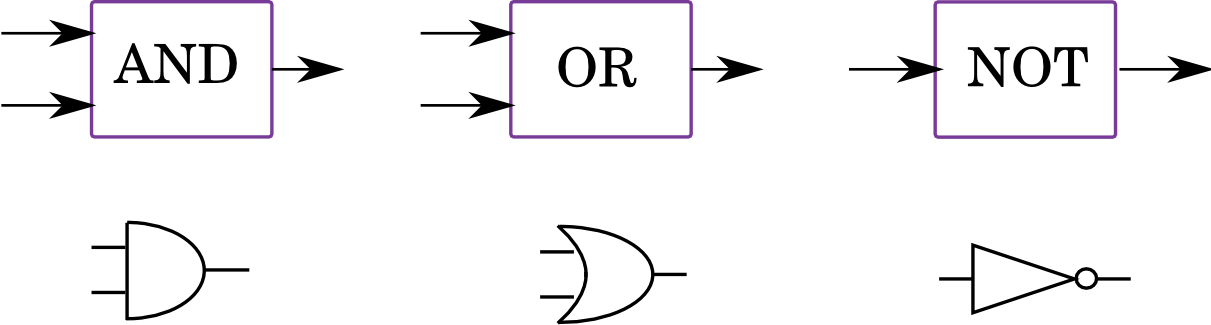
\includegraphics[width=0.25\paperwidth]{img/and}}
\par\end{centering}

\bigskip{}


\noindent \begin{centering}
\subfloat{\noindent \centering{}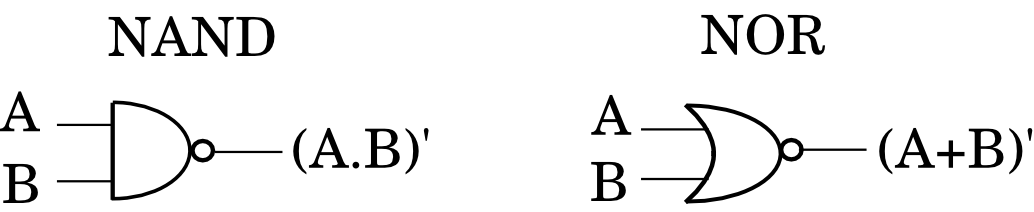
\includegraphics[width=0.25\textwidth]{img/nand}}
\par\end{centering}

\bigskip{}


\noindent \centering{}\subfloat{\noindent \centering{}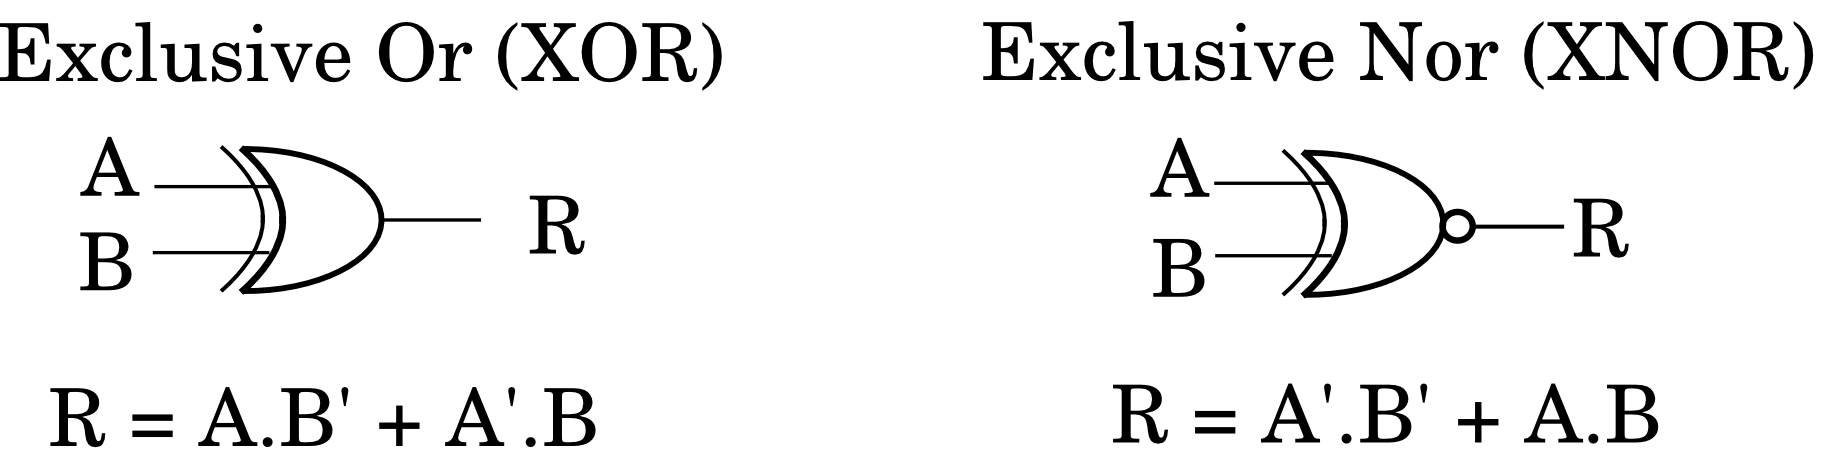
\includegraphics[width=0.25\paperwidth]{img/xor}}
\end{figure}



\paragraph{Analysing Circuits}

Work systematically, building up a formula or truth table in stages.


\paragraph{Simplifying Circuits}

Use De Morgan's:

\begin{figure}[H]
\noindent \centering{}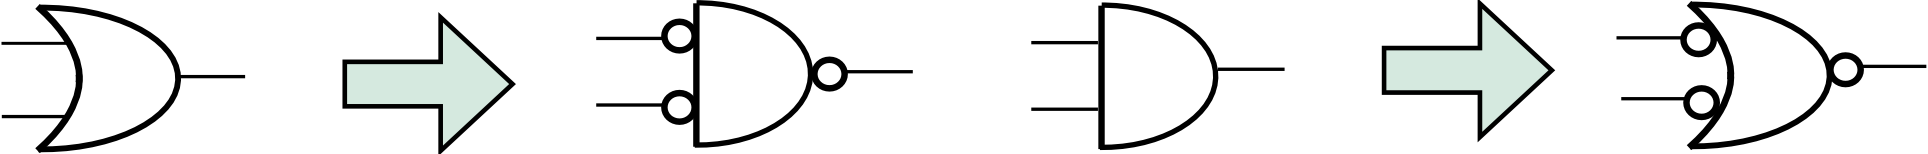
\includegraphics[width=0.25\paperwidth]{img/simplify}
\end{figure}



\paragraph{Control and Data Variables}

E.g. in a multiplexer:

\begin{figure}[H]
\noindent \centering{}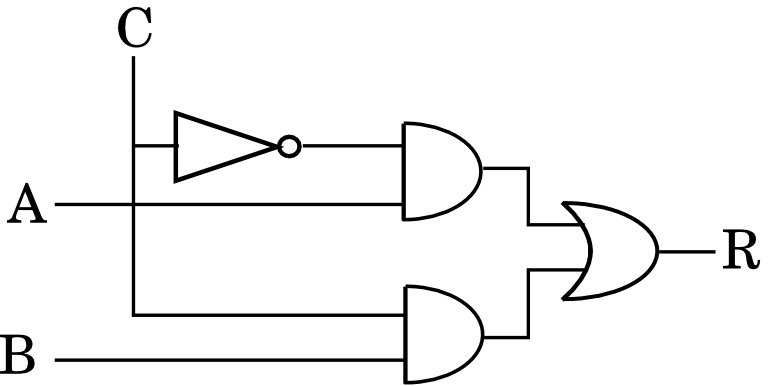
\includegraphics[width=0.15\paperwidth]{img/mux}
\end{figure}



\section{Combinatorial Circuits}


\paragraph{Minterms and Maxterms}
\begin{itemize}
\item \emph{Minterm}: Boolean product term in which for each input, $A_{k}$,
$A_{k}$ or $A_{k}'$ appears exactly once.
\item \emph{Maxterm}: Boolean sum term ....
\end{itemize}

\paragraph{Cannonical Forms}
\begin{itemize}
\item \emph{Minterm Cannonical Form}: Boolean sum of all minterms that ouput
1.
\item \emph{Maxterm Cannonical Form}: Boolean product of all maxterms that
output 0.
\end{itemize}

\paragraph{Karnaugh Maps}

E.g.

\begin{figure}[H]
\noindent \centering{}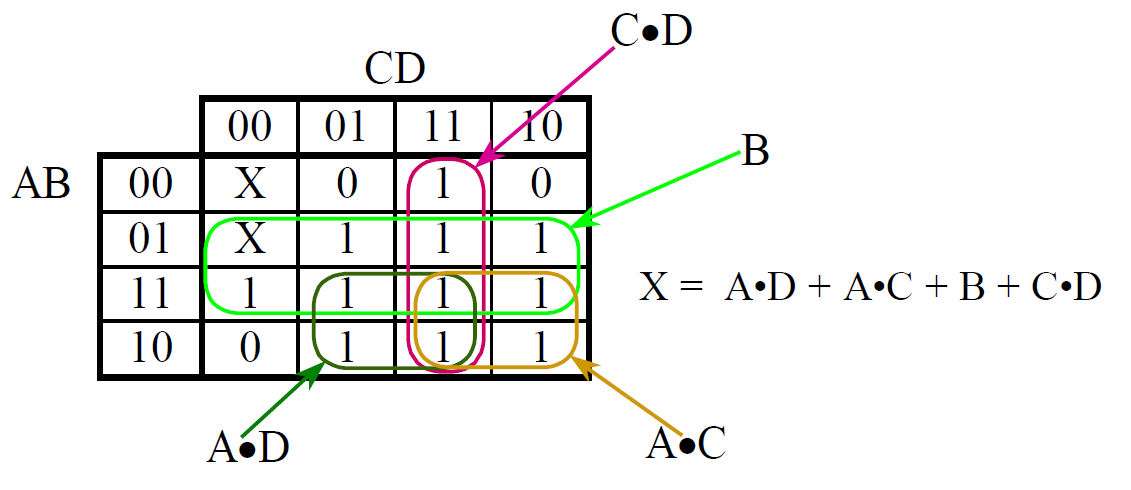
\includegraphics[width=0.25\paperwidth]{img/kmap}
\end{figure}


Remember:
\begin{itemize}
\item \emph{Order} (00, 01, 11, 10) is important.
\item K-maps are \emph{cyclic}.
\item We might be able to make a considerable simplification by considering
\emph{maxterms} (0s) instead of minterms.
\item \emph{Don't cares} (X) can be 0 or 1 - value depends on whether not
they are circled.
\end{itemize}

\paragraph{Combinatorial Circuit \emph{Design Process}}
\begin{enumerate}
\item Generate the truth table.
\item Generate the Karnaugh map.
\item Find the minimal Boolean Expression:

\begin{enumerate}
\item Read off the K-map.
\item Factor out any common factors.
\end{enumerate}
\item Draw the circuit.
\item Minimise to suit production method:

\begin{enumerate}
\item Reduce size (e.g. replace OR, AND by NOR, NAND).
\item Improve speed (reduce cycles).
\end{enumerate}
\item Test the circuit (e.g. systematic testing, formal verificaiton).
\end{enumerate}

\section{Physical Implementation}


\paragraph{Models of the Transistor}

Need to take into account a time delay.

\begin{table}[H]
\noindent \begin{minipage}[t]{0.1\textwidth}

\subfloat{\noindent \centering{}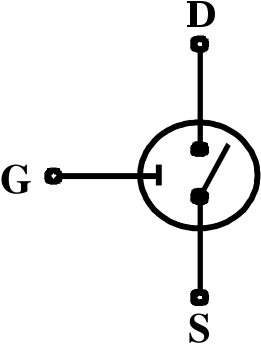
\includegraphics[width=0.08\paperwidth]{img/transistor-simple} }

\noindent \end{minipage}
\begin{minipage}[c]{0.4\textwidth}
\begin{enumerate}
\item \noindent \emph{Procedural model}:

\begin{enumerate}
\item $G,D$and $G,S$ not connected.
\item If $V_{GS}<0.5$V: switch open.
\item If $V_{GS}>1.7$V: switch closed.
\end{enumerate}
\item \emph{Time Delay}:

\begin{enumerate}
\item It takes a constant time for the transistor to which states - can
lead to spikes.
\end{enumerate}
\item \emph{Change is not Instantaneous}:

\begin{enumerate}
\item Account for capacitance: $I=C\frac{\mbox{d}V}{\mbox{d}t}$.
\end{enumerate}
\end{enumerate}
\noindent \centering{}\end{minipage}
\end{table}


Ideal change is 0 - 5V, but actually is somewhere close 0.2 - 3.7V
(with 0.5 - 1.7V considered non-deterministic).

\begin{figure}[H]
\noindent \centering{}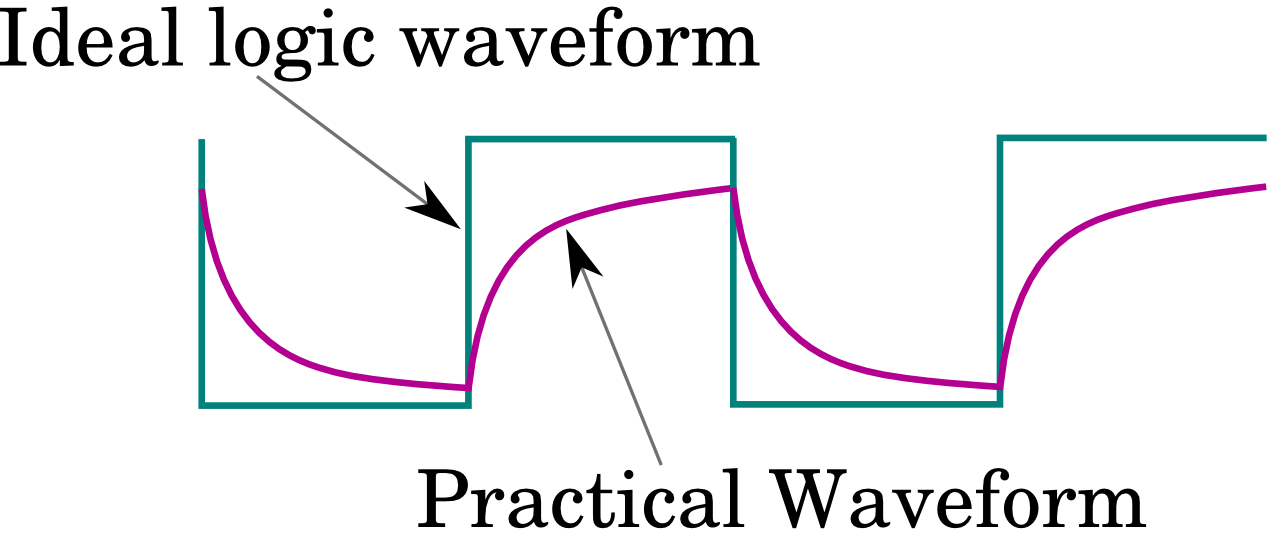
\includegraphics[width=0.15\paperwidth]{img/waveform}
\end{figure}


\begin{figure}[H]
\textbf{Basic Gate Implementations}

\noindent \begin{centering}
NOT
\par\end{centering}

\noindent \begin{centering}
\subfloat{\noindent \centering{}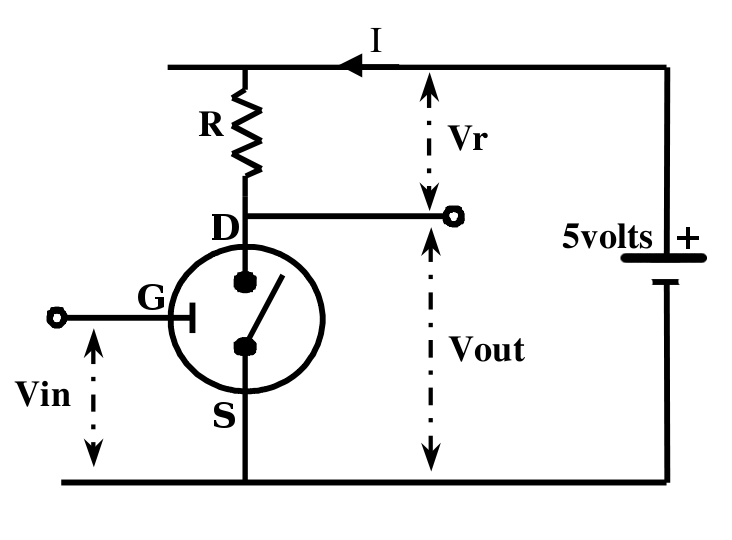
\includegraphics[width=0.2\paperwidth]{img/notgate}}
\par\end{centering}

\noindent \begin{centering}
NAND and NOR
\par\end{centering}

\noindent \centering{}\subfloat{\noindent \centering{}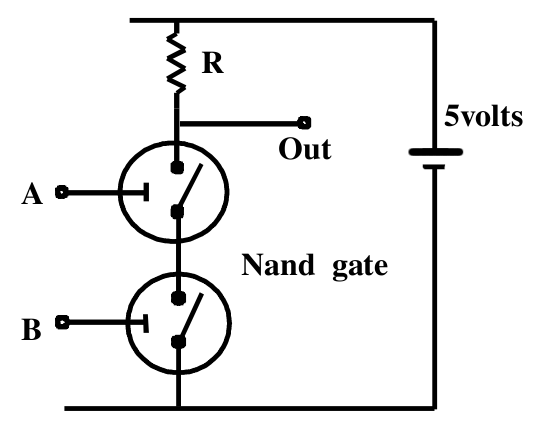
\includegraphics[width=0.15\textwidth]{img/nandgate}}\subfloat{\noindent \centering{}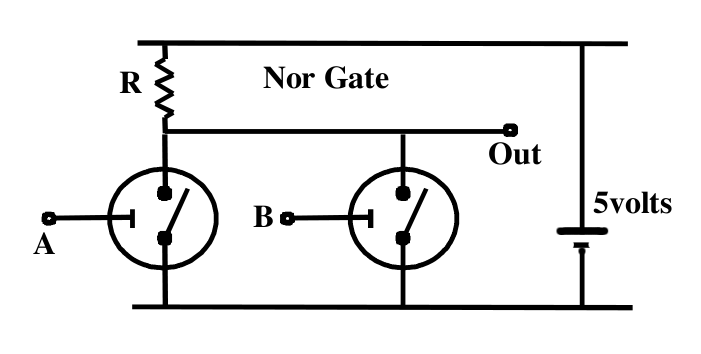
\includegraphics[width=0.175\paperwidth]{img/norgate}}
\end{figure}


Actual ICs generally use a combination of NMOS and PMOS (\textbf{C}omplimentary
\textbf{M}etal \textbf{O}xide \textbf{S}ilicon) instead of resistors
- lower power consumption and faster switching.

\begin{figure}[H]
\textbf{Time Dependent Behaviour of Circuits}

\noindent \centering{}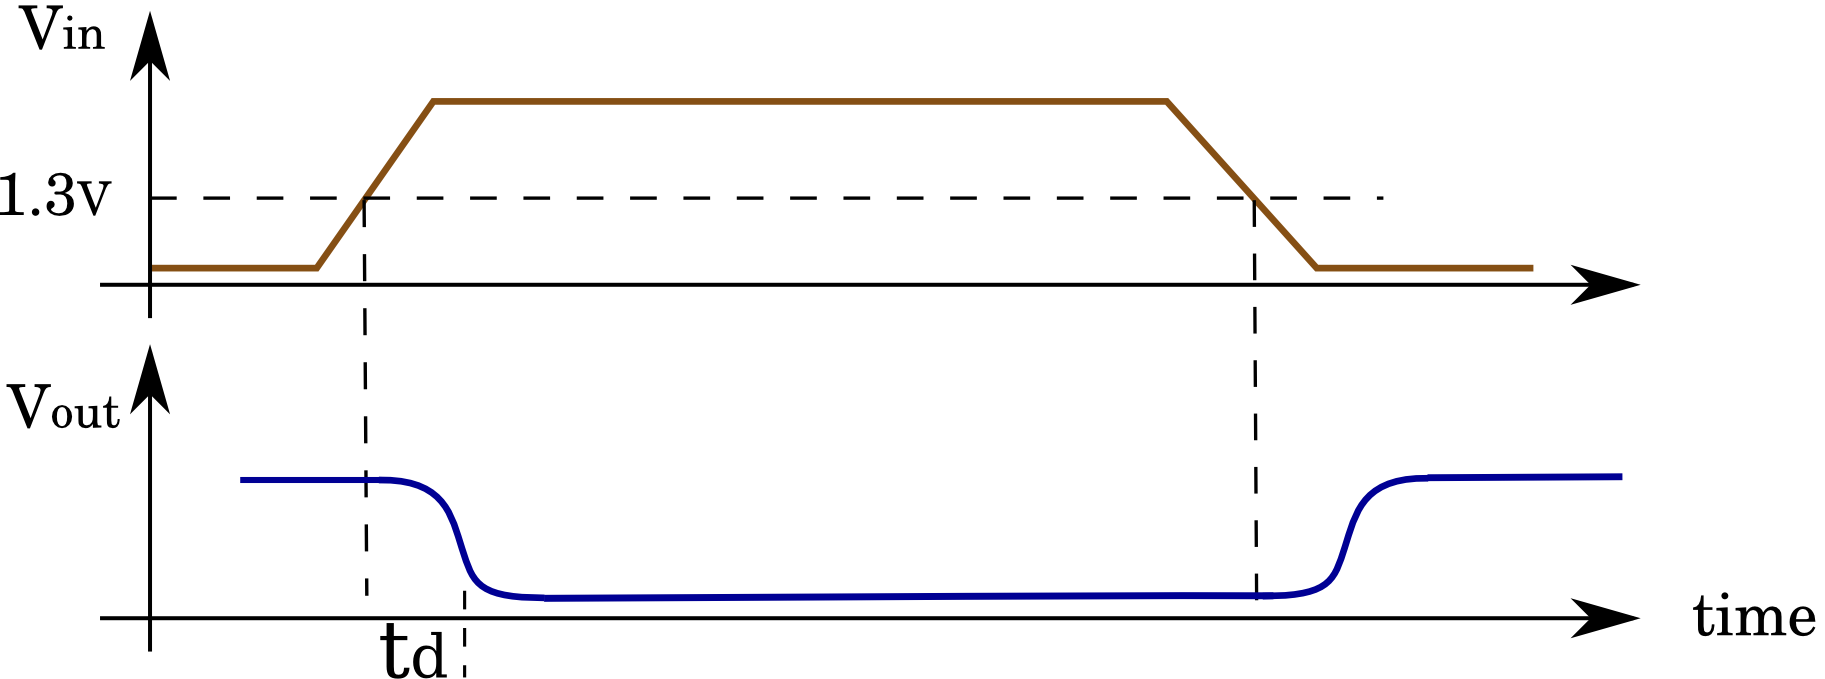
\includegraphics[width=0.25\paperwidth]{img/td}
\end{figure}


\begin{figure}[H]
\noindent \textbf{Noise Margin}

\noindent \centering{}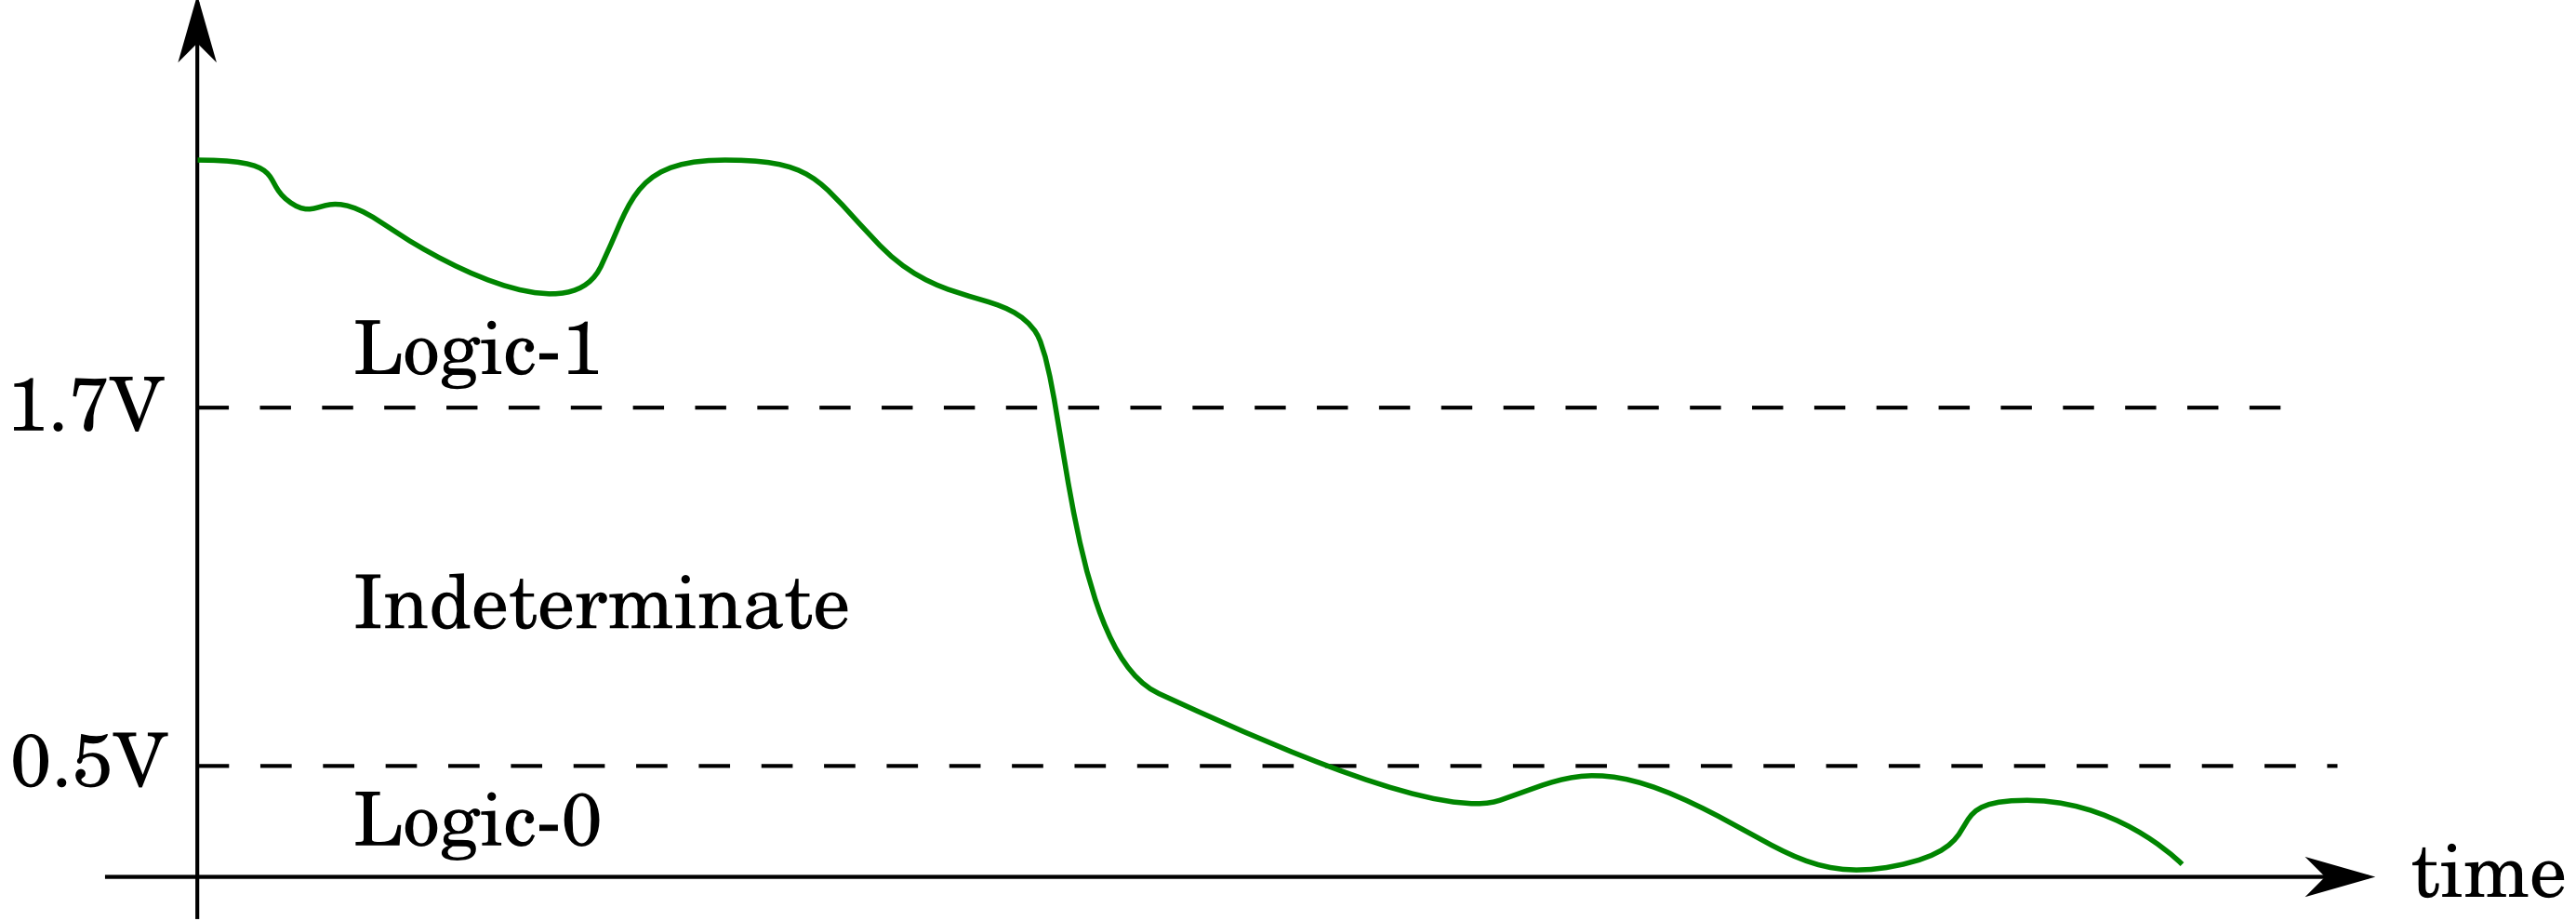
\includegraphics[width=0.3\paperwidth]{img/noise}
\end{figure}



\paragraph{Fan out}

The number of inputs to which the output of a gate is connected.
\begin{itemize}
\item Since $\frac{1}{R}=\frac{1}{R_{1}}+\frac{1}{R_{2}}+\dots+\frac{1}{R_{n}}$
for $n$ resistors in parallel, the load resistance decreases as fan
out increases, so output voltage falls.
\item Slows down circuit since capacitance is summed accross all gates.
\end{itemize}

\section{Synchronous Digital Systems}


\paragraph{Feedback}

Circuit below could:

\begin{figure}[H]
\noindent \centering{}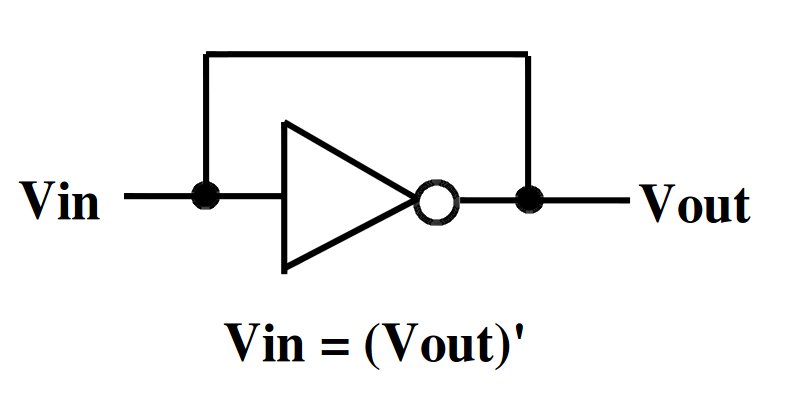
\includegraphics[width=0.1\paperwidth]{img/feedback}
\end{figure}

\begin{itemize}
\item Oscillate between values of 0 and 1.
\item Settle at an intermediate value (actually $\approx$1.2V).
\end{itemize}

\paragraph{Finite State Machine Representation}

E.g. consider:

\begin{figure}[H]
\noindent \centering{}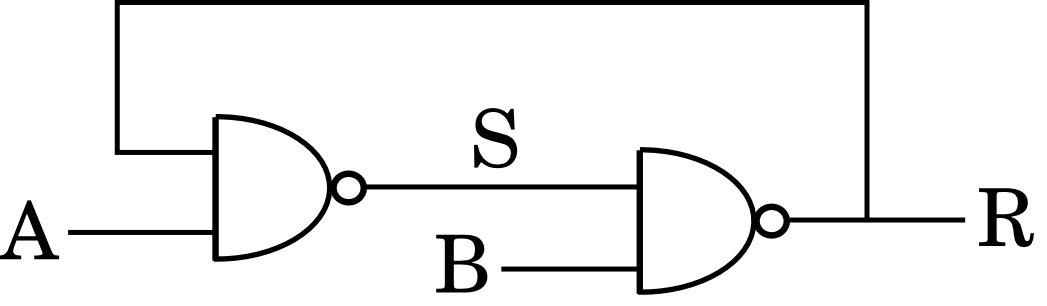
\includegraphics[width=0.15\paperwidth]{img/memcircuit}
\end{figure}


By considering all possible states for (ABSR) and what they lead to
in the following time step:

\begin{figure}[H]
\noindent \centering{}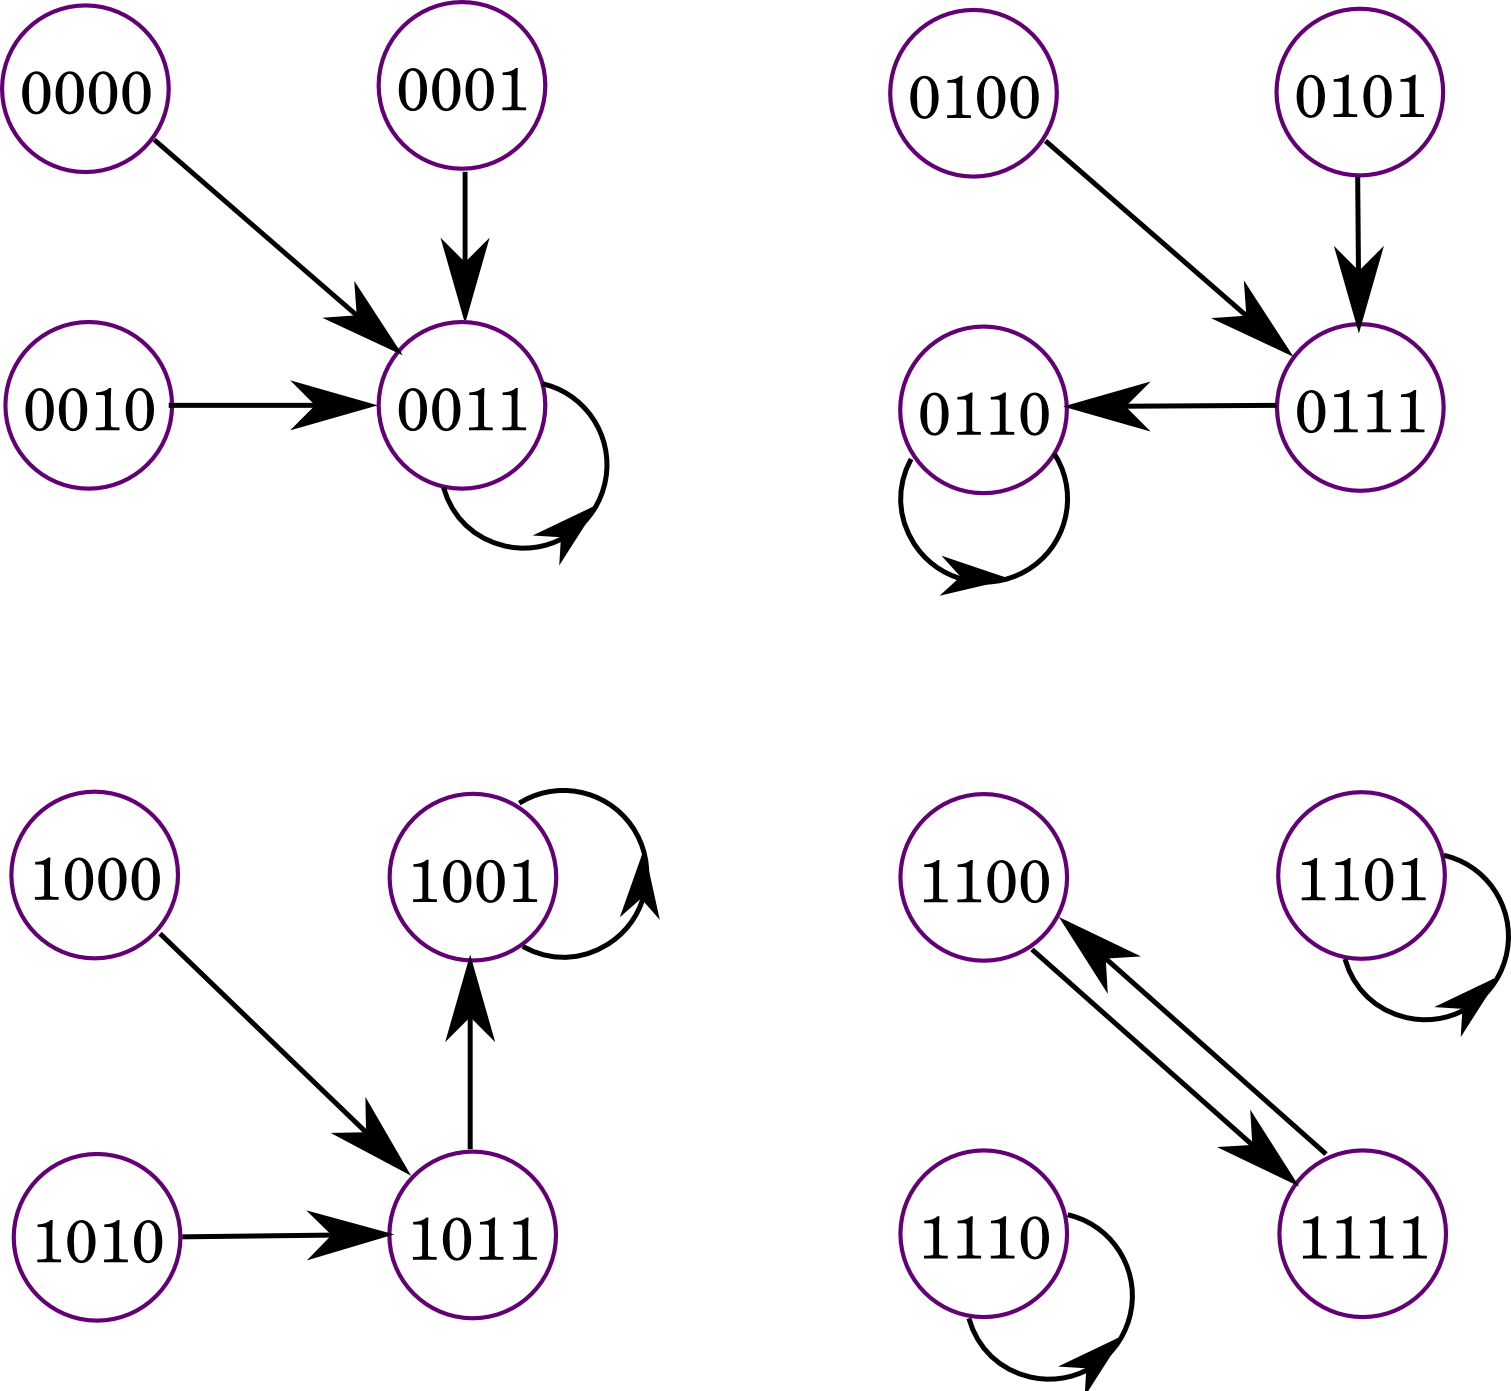
\includegraphics[width=0.25\paperwidth]{img/fsmr}
\end{figure}

\end{document}
